\documentclass{beamer}
\usetheme{Madrid}
\usecolortheme{whale}
\usepackage{amsmath}
\usepackage{amssymb}
\usepackage{physics}
\usepackage{tikz}
\usepackage{braket}
\usepackage{bm}
\title{From Symmetry to Computation: \
A Geometric Framework for Natural Information Processing}
\subtitle{Bridging Group Theory, Harmonic Analysis and Machine Learning}
\author{Ricardo Alexander Martinez}
\institute{Department of Computer Science\
Institution}
\date{\today}
\begin{document}
\begin{frame}
\titlepage
\end{frame}
\begin{frame}{Motivation}
\begin{itemize}
\item Current deep learning approaches:
\begin{itemize}
\item Quadratic attention complexity
\item Lack of geometric understanding
\item Resource inefficient
\end{itemize}
\item Nature suggests alternative:
\begin{itemize}
\item Symmetry-based computation
\item Hierarchical organization
\item Efficient pattern representation
\end{itemize}
\end{itemize}
\end{frame}
\begin{frame}{Rethinking Information Flow}
\begin{itemize}
\item Traditional Transformer Attention:
\begin{equation*}
O(n^2) \text{ comparisons for } n \text{ tokens}
\end{equation*}
\pause
\item Natural systems don't operate this way!
\end{itemize}
\end{frame}
\begin{frame}{Pattern Recognition Through Symmetry}
\begin{itemize}
\item Key Insight:
\begin{itemize}
\item Not about comparing everything
\item About detecting symmetries
\item Understanding transformations
\end{itemize}
\pause
\item Enter Spherical Harmonics:
\begin{equation*}
Y_l^m(\theta,\phi) \text{ - fundamental modes}
\end{equation*}
\end{itemize}
\end{frame}
\begin{frame}{Spherical Harmonics: Nature's Pattern Basis}
\begin{itemize}
\item Natural vibration modes of a sphere
\item Fundamental symmetric patterns
\item Properties:
\begin{itemize}
\item Orthogonal basis
\item Complete for square-integrable functions
\item Respect rotational symmetry
\end{itemize}
\end{itemize}
\begin{center}
\includegraphics[width=0.4\textwidth]{spherical_harmonics.png}
\end{center}
\end{frame}
\begin{frame}{From Harmonics to Lie Groups}
\begin{itemize}
\item Spherical Harmonic Decomposition:
\begin{equation*}
f(\theta,\phi) = \sum_{l=0}^{\infty}\sum_{m=-l}^l c_{lm}Y_l^m(\theta,\phi)
\end{equation*}
\item Not just representation, but transformation behavior!
\pause
\item Connection to Lie Groups:
\begin{equation*}
\text{SO}(3) \text{ generators } \leftrightarrow \text{ rotational patterns}
\end{equation*}
\end{itemize}
\end{frame}
\begin{frame}{Hardware Implementation}
\begin{itemize}
\item RTX 4080 Specifications:
\begin{itemize}
\item 9728 CUDA cores
\item 717 GB/s memory bandwidth
\item Effective throughput: $\approx 430$ GB/s
\end{itemize}
\item Parallel Processing:
\begin{equation*}
\text{Core}_{i,j} \rightarrow (l_i,m_j) \text{ harmonic pair}
\end{equation*}
\end{itemize}
\end{frame}
\begin{frame}{Memory Hierarchy Design}
\begin{center}
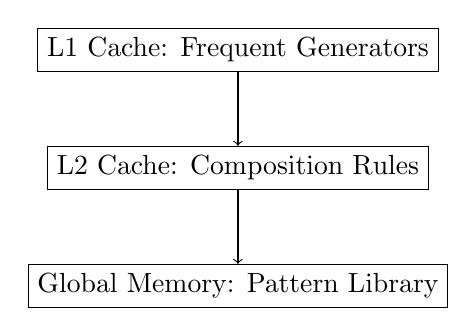
\begin{tikzpicture}[node distance=1.5cm]
\node[draw,rectangle] (l1) {L1 Cache: Frequent Generators};
\node[draw,rectangle,below of=l1] (l2) {L2 Cache: Composition Rules};
\node[draw,rectangle,below of=l2] (global) {Global Memory: Pattern Library};
\draw[->] (l1) -- (l2);
\draw[->] (l2) -- (global);
\end{tikzpicture}
\end{center}
\begin{itemize}
\item Natural alignment with computation flow
\item Optimal cache utilization
\item Hierarchical pattern storage
\end{itemize}
\end{frame}
\begin{frame}{Complexity Analysis}
\begin{table}
\begin{tabular}{lll}
\hline
Operation & Traditional & Our Approach \
\hline
Computation & $O(n^2)$ & $O(L \log L)$ \
Memory & $O(n^2)$ & $O(\log k)$ \
Pattern Matching & $O(n^2)$ & $O(\log k)$ \
\hline
\end{tabular}
\caption{$n$: sequence length, $L$: harmonic degree, $k$: unique patterns}
\end{table}
\end{frame}
\begin{frame}{Spinor Structure Emergence}
\begin{itemize}
\item Natural consequence of 3D rotations:
\begin{equation*}
\text{SU}(2) \xrightarrow{2:1} \text{SO}(3)
\end{equation*}
\pause
\item Quaternion representation:
\begin{equation*}
q = a + bi + cj + dk
\end{equation*}
\begin{itemize}
\item 4 components vs 9 for matrices
\item Better numerical stability
\item Natural composition
\end{itemize}
\end{itemize}
\end{frame}
\begin{frame}{Geometric Insights}
\begin{center}
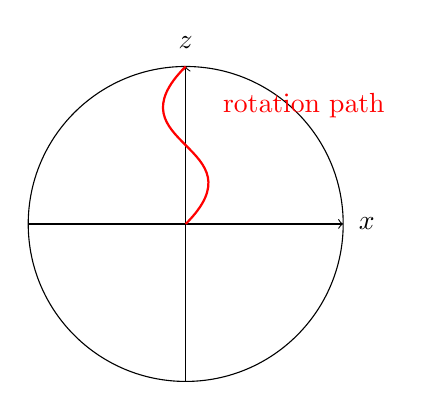
\begin{tikzpicture}
\draw (0,0) circle (2cm);
\draw[->] (-2,0) -- (2,0);
\draw[->] (0,-2) -- (0,2);
\node at (2.3,0) {$x$};
\node at (0,2.3) {$z$};
\draw[red,thick] (0,0) .. controls (1,1) and (-1,1) .. (0,2);
\node[red] at (1.5,1.5) {rotation path};
\end{tikzpicture}
\end{center}
\begin{itemize}
\item Double cover ensures continuous paths
\item Quaternions avoid gimbal lock
\item Natural representation of rotations
\end{itemize}
\end{frame}
\begin{frame}{Cache Coherency Through Harmonic Locality}
\begin{itemize}
\item Frequency-space locality:
\begin{equation*}
Y_l^m \text{ and } Y_{l\pm1}^{m\pm1} \text{ are spatially related}
\end{equation*}
\item Memory layout follows harmonic structure:
\begin{center}
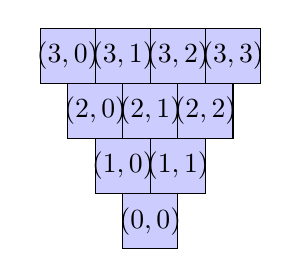
\begin{tikzpicture}[scale=0.7]
\foreach \x in {0,...,3} {
\foreach \y in {0,...,\x} {
\draw[fill=blue!20] (\y-\x/2,\x) rectangle ++(1,1);
\node at (\y-\x/2+0.5,\x+0.5) {$(\x,\y)$};
}
}
\end{tikzpicture}
\end{center}
\end{itemize}
\end{frame}
\begin{frame}{GPU Implementation}
\begin{itemize}
\item Compute Shader Organization:
\begin{itemize}
\item Warp = Natural group boundary
\item Shared memory = Local transformations
\item Coalesced access patterns
\end{itemize}
\pause
\item Synchronization:
\begin{equation*}
\text{barrier}(\text{GROUP_SHARED_MEMORY})
\end{equation*}
\end{itemize}
\end{frame}
\begin{frame}{Numerical Stability}
\begin{itemize}
\item Near-pole stability:
\begin{equation*}
\text{precision}(\theta) = \begin{cases}
\text{double}, & |\theta| < \epsilon \
\text{float}, & \text{otherwise}
\end{cases}
\end{equation*}
\item Error correction through group structure:
\begin{equation*}
g' = \text{normalize}(g) \in \text{SU}(2)
\end{equation*}
\end{itemize}
\end{frame}
\begin{frame}{Git Analogy: Continuous Geometric Version}
\begin{center}
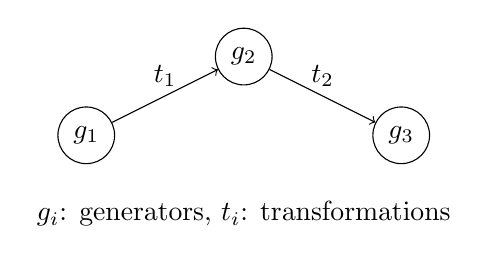
\begin{tikzpicture}
\node[draw,circle] (A) at (0,0) {$g_1$};
\node[draw,circle] (B) at (2,1) {$g_2$};
\node[draw,circle] (C) at (4,0) {$g_3$};
\draw[->] (A) -- node[above] {$t_1$} (B);
\draw[->] (B) -- node[above] {$t_2$} (C);
\node at (2,-1) {$g_i$: generators, $t_i$: transformations};
\end{tikzpicture}
\end{center}
\begin{itemize}
\item Store generators instead of states
\item Minimal representation
\item Natural composition through group structure
\end{itemize}
\end{frame}
\begin{frame}{Natural Information Processing}
\begin{itemize}
\item Key Realization:
\begin{itemize}
\item Not just an implementation trick
\item Fundamental principle of physical systems
\item Mathematics reflects natural computation
\end{itemize}
\pause
\item Unified View:
\begin{equation*}
\text{Math} \leftrightarrow \text{Computation} \leftrightarrow \text{Physics}
\end{equation*}
\end{itemize}
\end{frame}
\begin{frame}{Biological Information Processing}
\begin{itemize}
\item Head rotation example:
\begin{itemize}
\item No explicit matrix multiplication
\item Direct symmetry detection
\item Continuous update of orientation
\end{itemize}
\pause
\item Natural System Properties:
\begin{equation*}
\text{Local} \rightarrow \text{Global} \text{ through symmetry}
\end{equation*}
\end{itemize}
\end{frame}
\begin{frame}{Pattern Trajectories in Lie Groups}
\begin{center}
\begin{tikzpicture}
\draw[->] (-2,0) -- (2,0) node[right] {$x$};
\draw[->] (0,-2) -- (0,2) node[above] {$y$};
\draw[red,thick] plot[domain=0:2pi,samples=100]
({cos(\x r)},{sin(\x r)});
\node[red] at (1.5,1.5) {$SO(3)$ trajectory};
\end{tikzpicture}
\end{center}
\begin{equation*}
\text{Pattern}(t) = e^{tX}\text{Pattern}(0), \quad X \in \mathfrak{so}(3)
\end{equation*}
\begin{itemize}
\item Patterns as paths in transformation space
\item Continuous morphing through group action
\item Natural geodesics in pattern space
\end{itemize}
\end{frame}
\begin{frame}{Beyond Parallel Processing}
\begin{itemize}
\item Hardware Resources:
\begin{itemize}
\item RTX 4080: 9728 cores
\item Naive approach: One core per harmonic component
\end{itemize}
\pause
\item Key Insight:
\begin{equation*}
\text{Storage} \propto \dim(\mathfrak{g}) \ll \dim(G)
\end{equation*}
where $\mathfrak{g}$ is the Lie algebra, $G$ is the group
\end{itemize}
\end{frame}
\begin{frame}{Natural Compression Through Group Structure}
\begin{center}
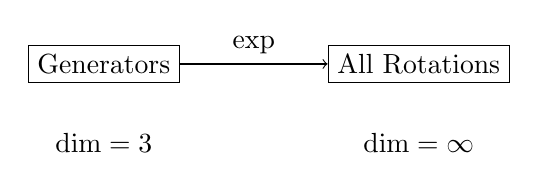
\begin{tikzpicture}
\node[draw,rectangle] (gen) at (0,0) {Generators};
\node[draw,rectangle] (rot) at (4,0) {All Rotations};
\draw[->] (gen) -- node[above] {$\exp$} (rot);
\node at (0,-1) {$\dim = 3$};
\node at (4,-1) {$\dim = \infty$};
\end{tikzpicture}
\end{center}
\begin{equation*}
R(\theta) = e^{\theta X}, \quad X \in \mathfrak{so}(3)
\end{equation*}
\end{frame}
\begin{frame}{Git Analogy Deepens}
\begin{columns}
\column{0.5\textwidth}
Git Version Control:
\begin{itemize}
\item Stores diffs, not states
\item Minimal change representation
\item Composition of changes
\end{itemize}
 \column{0.5\textwidth}
    Lie Group Structure:
    \begin{itemize}
        \item Stores generators
        \item Minimal transformation basis
        \item Group composition
    \end{itemize}
\end{columns}
\begin{equation*}
    \text{commit} \sim e^X, \quad X \in \mathfrak{g}
\end{equation*}
\end{frame}
\begin{frame}{Natural Memory Hierarchy}
\begin{center}
\begin{tikzpicture}[node distance=2cm]
\node[draw,rectangle,fill=blue!20] (l1) {L1: Generators};
\node[draw,rectangle,fill=green!20,below of=l1] (l2) {L2: Composition Rules};
\node[draw,rectangle,fill=red!20,below of=l2] (l3) {L3: Pattern Families};
\draw[->] (l1) -- node[right] {generates} (l2);
\draw[->] (l2) -- node[right] {organizes} (l3);
\node[draw,ellipse,right of=l3] (orbit) {Orbit Structure};
        \draw[->] (l3) -- node[above] {induces} (orbit);
    \end{tikzpicture}
\end{center}
\begin{equation*}
    \text{Pattern Family} = \{g \cdot p \mid g \in G\}
\end{equation*}
\end{frame}
\begin{frame}{Double-Cover Structure Revisited}
\begin{itemize}
\item Beyond Rotation:
\begin{equation*}
\text{SU}(2) \xrightarrow{2:1} \text{SO}(3)
\end{equation*}
\item Information Organization:
\begin{itemize}
\item Natural double-cover emergence
\item Quantum mechanical parallel
\item Topological protection
\end{itemize}
\pause
\item Universal Principle:
\begin{equation*}
\text{Spin Structure} \rightarrow \text{Information Structure}
\end{equation*}
\end{itemize}
\end{frame}
\begin{frame}{Singularity Management}
\begin{itemize}
\item Group-Theoretic Approach:
\begin{equation*}
\text{Stability}(p) = \begin{cases}
\text{Use generators}, & p \text{ near pole} \
\text{Direct computation}, & \text{otherwise}
\end{cases}
\end{equation*}
\pause
\item Control System Analogy:
\begin{itemize}
\item Natural feedback loops
\item Automatic error correction
\item Geometric regularization
\end{itemize}
\end{itemize}
\end{frame}
\begin{frame}{Edge Case Handling}
\begin{center}
\begin{tikzpicture}
\draw[->] (-2,0) -- (2,0) node[right] {$x$};
\draw[->] (0,-2) -- (0,2) node[above] {$y$};
\draw[red,thick] plot[domain=-pi/2:pi/2,samples=100]
({tan(\x r)},{1/cos(\x r)});
\node[red] at (1.5,1.5) {singular region};
\draw[blue,thick] (0,0) circle (0.3);
\node[blue] at (0.5,0.3) {stable region};
\end{tikzpicture}
\end{center}
\begin{itemize}
\item Group structure provides natural regularization
\item Automatic handling of coordinate singularities
\item Smooth transition between computational regimes
\end{itemize}
\end{frame}
\begin{frame}{CUDA Implementation Details}
\begin{itemize}
\item Core Assignment:
\begin{equation*}
\text{CUDA}_i \mapsto (l_i, m_i) \text{ where } |m_i| \leq l_i
\end{equation*}
\item Memory Organization:
\begin{itemize}
\item Bandwidth: 717 GB/s
\item Cache line size: 128 bytes
\item Natural alignment with $(l,m)$ boundaries
\end{itemize}
\end{itemize}
\end{frame}
\begin{frame}{Natural Computation Structure}
\begin{center}
\begin{tikzpicture}
\foreach \x in {0,...,3} {
\foreach \m in {-\x,...,\x} {
\node[draw,circle,fill=blue!\the\numexpr70-\x20\relax]
at (\m1.5,\x1.2) {$(\x,\m)$};
}
}
\draw[->] (0,0) -- (1.5,1.2);
\draw[->] (-1.5,1.2) -- (0,2.4);
\end{tikzpicture}
\end{center}
\begin{equation*}
\text{Cache Line} \sim \text{Natural Frequency Band}
\end{equation*}
\end{frame}
\begin{frame}{Geometric Attention}
\begin{itemize}
\item Traditional Attention:
\begin{equation*}
A(Q,K,V) = \text{softmax}\left(\frac{QK^T}{\sqrt{d}}\right)V
\end{equation*}
\pause
\item Geometric Alternative:
\begin{equation*}
A_G(x,y) = \int_G K(g \cdot x, y) , dg
\end{equation*}
where $G$ is our transformation group
\end{itemize}
\end{frame}
\begin{frame}{Natural Pathways in Transformation Space}
\begin{center}
\begin{tikzpicture}
\draw[->] (-2,0) -- (2,0) node[right] {$x$};
\draw[->] (0,-2) -- (0,2) node[above] {$y$};
\draw[red,thick] plot[domain=0:2pi,samples=100]
({cos(\x r)},{sin(\x r)});
\draw[blue,thick] plot[domain=0:pi,samples=50]
({2cos(\x r)},{sin(\x r)});
\node at (1.5,1.5) {transformation paths};
\end{tikzpicture}
\end{center}
\begin{itemize}
\item Attention emerges from geometry
\item Natural geodesics in pattern space
\item Efficient path discovery
\end{itemize}
\end{frame}
\end{document}